% -*- Mode:TeX -*-

%% IMPORTANT: The official thesis specifications are available at:
%%            http://libraries.mit.edu/archives/thesis-specs/
%%
%%            Please verify your thesis' formatting and copyright
%%            assignment before submission.  If you notice any
%%            discrepancies between these templates and the 
%%            MIT Libraries' specs, please let us know
%%            by e-mailing thesis@mit.edu

%% The documentclass options along with the pagestyle can be used to generate
%% a technical report, a draft copy, or a regular thesis.  You may need to
%% re-specify the pagestyle after you \include  cover.tex.  For more
%% information, see the first few lines of mitthesis.cls. 

%\documentclass[12pt,vi,twoside]{mitthesis}
%%
%%  If you want your thesis copyright to you instead of MIT, use the
%%  ``vi'' option, as above.
%%
%\documentclass[12pt,twoside,leftblank]{mitthesis}
%%
%% If you want blank pages before new chapters to be labelled ``This
%% Page Intentionally Left Blank'', use the ``leftblank'' option, as
%% above. 

\documentclass[12pt,twoside]{mitthesis}
\usepackage{lgrind}
\pagestyle{plain}

%% This bit allows you to either specify only the files which you wish to
%% process, or `all' to process all files which you \include.
%% Krishna Sethuraman (1990).

\typein [\files]{Enter file names to process, (chap1,chap2 ...), or `all' to
process all files:}
\def\all{all}
\ifx\files\all \typeout{Including all files.} \else \typeout{Including only \files.} \includeonly{\files} \fi

\begin{document}

% -*-latex-*-
% 
% For questions, comments, concerns or complaints:
% thesis@mit.edu
% 
%
% $Log: cover.tex,v $
% Revision 1.8  2008/05/13 15:02:15  jdreed
% Degree month is June, not May.  Added note about prevdegrees.
% Arthur Smith's title updated
%
% Revision 1.7  2001/02/08 18:53:16  boojum
% changed some \newpages to \cleardoublepages
%
% Revision 1.6  1999/10/21 14:49:31  boojum
% changed comment referring to documentstyle
%
% Revision 1.5  1999/10/21 14:39:04  boojum
% *** empty log message ***
%
% Revision 1.4  1997/04/18  17:54:10  othomas
% added page numbers on abstract and cover, and made 1 abstract
% page the default rather than 2.  (anne hunter tells me this
% is the new institute standard.)
%
% Revision 1.4  1997/04/18  17:54:10  othomas
% added page numbers on abstract and cover, and made 1 abstract
% page the default rather than 2.  (anne hunter tells me this
% is the new institute standard.)
%
% Revision 1.3  93/05/17  17:06:29  starflt
% Added acknowledgements section (suggested by tompalka)
% 
% Revision 1.2  92/04/22  13:13:13  epeisach
% Fixes for 1991 course 6 requirements
% Phrase "and to grant others the right to do so" has been added to 
% permission clause
% Second copy of abstract is not counted as separate pages so numbering works
% out
% 
% Revision 1.1  92/04/22  13:08:20  epeisach

% NOTE:
% These templates make an effort to conform to the MIT Thesis specifications,
% however the specifications can change.  We recommend that you verify the
% layout of your title page with your thesis advisor and/or the MIT 
% Libraries before printing your final copy.
\title{InMind: Mobile Application for Sharing the Status of Serious Stuff}

\author{Joy C. Chen}
% If you wish to list your previous degrees on the cover page, use the 
% previous degrees command:
%       \prevdegrees{A.A., Harvard University (1985)}
% You can use the \\ command to list multiple previous degrees
%       \prevdegrees{B.S., University of California (1978) \\
%                    S.M., Massachusetts Institute of Technology (1981)}
\department{Department of Electrical Engineering and Computer Science}

% If the thesis is for two degrees simultaneously, list them both
% separated by \and like this:
% \degree{Doctor of Philosophy \and Master of Science}
\degree{Bachelor of Science \and Master of Science in Computer Science and Engineering}

% As of the 2007-08 academic year, valid degree months are September, 
% February, or June.  The default is June.
\degreemonth{June}
\degreeyear{2014}
\thesisdate{May 23, 2014}

%% By default, the thesis will be copyrighted to MIT.  If you need to copyright
%% the thesis to yourself, just specify the `vi' documentclass option.  If for
%% some reason you want to exactly specify the copyright notice text, you can
%% use the \copyrightnoticetext command.  
%\copyrightnoticetext{\copyright IBM, 1990.  Do not open till Xmas.}

% If there is more than one supervisor, use the \supervisor command
% once for each.
\supervisor{Rosalind Picard}{Professor of Media Arts and Sciences}

% This is the department committee chairman, not the thesis committee
% chairman.  You should replace this with your Department's Committee
% Chairman.
\chairman{Albert Meyer}{Chairman, Department Committee on Graduate Theses}

% Make the titlepage based on the above information.  If you need
% something special and can't use the standard form, you can specify
% the exact text of the titlepage yourself.  Put it in a titlepage
% environment and leave blank lines where you want vertical space.
% The spaces will be adjusted to fill the entire page.  The dotted
% lines for the signatures are made with the \signature command.
\maketitle

% The abstractpage environment sets up everything on the page except
% the text itself.  The title and other header material are put at the
% top of the page, and the supervisors are listed at the bottom.  A
% new page is begun both before and after.  Of course, an abstract may
% be more than one page itself.  If you need more control over the
% format of the page, you can use the abstract environment, which puts
% the word "Abstract" at the beginning and single spaces its text.

%% You can either \input (*not* \include) your abstract file, or you can put
%% the text of the abstract directly between the \begin{abstractpage} and
%% \end{abstractpage} commands.

% First copy: start a new page, and save the page number.
\cleardoublepage
% Uncomment the next line if you do NOT want a page number on your
% abstract and acknowledgments pages.
% \pagestyle{empty}
\setcounter{savepage}{\thepage}
\begin{abstractpage}
% $Log: abstract.tex,v $
%
%% The text of your abstract and nothing else (other than comments) goes here.
%% It will be single-spaced and the rest of the text that is supposed to go on
%% the abstract page will be generated by the abstractpage environment.  This
%% file should be \input (not \include 'd) from cover.tex.

TBD

\end{abstractpage}

% Additional copy: start a new page, and reset the page number.  This way,
% the second copy of the abstract is not counted as separate pages.
% Uncomment the next 6 lines if you need two copies of the abstract
% page.
% \setcounter{page}{\thesavepage}
% \begin{abstractpage}
% % $Log: abstract.tex,v $
%
%% The text of your abstract and nothing else (other than comments) goes here.
%% It will be single-spaced and the rest of the text that is supposed to go on
%% the abstract page will be generated by the abstractpage environment.  This
%% file should be \input (not \include 'd) from cover.tex.

TBD

% \end{abstractpage}

\cleardoublepage

\section*{Acknowledgments}
TBD!
Roz, JofishK, MMassimi,
Craig, Micah
Elliott, Rob.

All my interviewees!

%%%%%%%%%%%%%%%%%%%%%%%%%%%%%%%%%%%%%%%%%%%%%%%%%%%%%%%%%%%%%%%%%%%%%%
% -*-latex-*-

% Some departments (e.g. 5) require an additional signature page.  See
% signature.tex for more information and uncomment the following line if
% applicable.
% % -*- Mode:TeX -*-
%
% Some departments (e.g. Chemistry) require an additional cover page
% with signatures of the thesis committee.  Please check with your
% thesis advisor or other appropriate person to determine if such a 
% page is required for your thesis.  
%
% If you choose not to use the "titlepage" environment, a \newpage
% commands, and several \vspace{\fill} commands may be necessary to
% achieve the required spacing.  The \signature command is defined in
% the "mitthesis" class
%
% The following sample appears courtesy of Ben Kaduk <kaduk@mit.edu> and
% was used in his June 2012 doctoral thesis in Chemistry. 

\begin{titlepage}
\begin{large}
This doctoral thesis has been examined by a Committee of the Department
of Chemistry as follows:

\signature{Professor Jianshu Cao}{Chairman, Thesis Committee \\
   Professor of Chemistry}

\signature{Professor Troy Van Voorhis}{Thesis Supervisor \\
   Associate Professor of Chemistry}

\signature{Professor Robert W. Field}{Member, Thesis Committee \\
   Haslam and Dewey Professor of Chemistry}
\end{large}
\end{titlepage}


\pagestyle{plain}
  % -*- Mode:TeX -*-
%% This file simply contains the commands that actually generate the table of
%% contents and lists of figures and tables.  You can omit any or all of
%% these files by simply taking out the appropriate command.  For more
%% information on these files, see appendix C.3.3 of the LaTeX manual. 
\tableofcontents
\newpage
\listoffigures
\newpage
\listoftables


%% This is an example first chapter.  You should put chapter/appendix that you
%% write into a separate file, and add a line \include{yourfilename} to
%% main.tex, where `yourfilename.tex' is the name of the chapter/appendix file.
%% You can process specific files by typing their names in at the 
%% \files=
%% prompt when you run the file main.tex through LaTeX.
\chapter{Introduction}
  Social support is an important resource during times of transition and stress.
  Whether it's friends, collegues, families, or anyone else, the people in our lives
  are what help get us through difficult transitions.
  \cite{mikal13}
  The impact of this support has manifested itself in a broad range of studies.
  Rains and Young found that supportive communication can help manage uncertainty and
  help one feel in control of one's life \cite{rains09},
  and Shor et all even discovered that support from
  family is correlated with lower mortality. \cite{shor13}

  However, as the complexity of personal networks suggests, the resources that people pull on
  are very specific,
  and their appropriateness is a complex subject.
  It is thus important to recognize that not all support is the same.
  Lehman et al studied in 1986 the ways that attempts at support that were helpful and unhelpful.
  \cite{lehman86}
  When Vachon and Stylianos explored the "goodness of fit" between offered support and the actual needs of
  the bereaved, they discovered that it varies wildly, and is sensitive to variables such as impact of loss
  and presence of other stressors.
  \cite{vachon88}
  
  Further, stressful transition periods can be accompanied by changes in the social structure
  that the support depends upon.
  The situation of illness or bereavement obviously includes, necessarily,
  the loss of an individual that would otherwise be a source of support,
  but many other transitions can also cause rearrangement of personal networks.
  Consequently, during transitions is often when these much needed
  support mechanisms can weaken or fail.
  \cite{mikal13}

  In this thesis, I am interested in exploring
  the ways that technology actually helps individuals going
  through stressful transitions.

  This work fits into the broader universe of
  recent Human Computer Interaction research
  done to address the need to mediate social support
  and other forms of intimacy through technology.
  \cite{hassenzhal12}
  Technology can help to mediate the appropriate type of resilient support
  that individuals may need.
  Promisingly, there has been significant evidence that
  mobile and web based social interactions can have positive effects similar
  to more traditional social interactions.
  \cite{??}

\section{Overview}
  The work of this thesis is split into roughly three different areas.
  \begin{enumerate}
  \item \textbf{Interviews and Questionnaires} were conducted to better understand
    university students' existing interaction with intimate socials
    such as family or friends while going through a stressful period in life.
  \item \textbf{Field Tests} of a technological probe, the InMind Android application,
    over 3 weeks
    explore the concept of a life issue tracker that is shared with friends.
    Data that was logged was used to answer questions about privacy choices that users make.
  \item \textbf{Feedback and Reflection} on the usage of the InMind application,
    as well as the evolving nature of the participant' situations will
    be used to motivate future design.
  \end{enumerate}

\section{Project Vision and History}
\label{sec:vision}
  InMind began as an application designed to help bereaved individuals deal with
  some of their specific needs, specifically story, affect, and availability sharing.

  My initial prototype, InMourning, targeted three needs that became apparent
  from needfinding studies conducted by Massimi and
  Baecker \cite{mm11a, mm10, mm13},

  \begin{enumerate}
  \item \textbf{Affect Sharing} - The well being of bereaved individuals is often a subject
    of inquiry, and sharing this information is a common task.
  \item \textbf{Availability Sharing} -
    Caring friends and family often want to be present
    and available for the bereaved, however,
    the bereaved generally want to control the nature and timing of communication between
    them and their family, friends, and other supporters.
    The bereaved are sensitive to what kind
    of interaction (texts, calls, face-to-face visits) and when they occur (exactly
    what hour of what day, or frequency). The influx of media and ways to
    communicate actually make it consistently overwhelming for the bereaved,
    particularly added to the already stressful interactions that necessarily
    follow a loved one's passing.
    Thus, the availability of the bereaved, how able and willing they are
    to accommodate guests, is important to communicate.
  \item \textbf{Story Sharing} - Bereaved individuals feel a need to share stories related to
    or inspired by their relationship with the departed.
    From reflecting on a trigger, pattern, or thought that carries unusual
    significance for the mourner to full blown story telling, bereaved individuals
    consistently want to share aspects of their experience with caring friends and
    family, many of whom are likely mourning the same loss.
  \end{enumerate}

  These three needs were collected because they addressed the common theme of improving
  relationships with caring friends and family during the time of difficulty.

  In the context of these needs, I developed InMourning to work in an HCI study,
  in the theme of existing bereavement technologies,
  hoping to better understand how people can use technology to meet their needs.
  The initial prototypes of InMourning are attached to this in Appendix C.

  However, the more we explored the needs of bereaved individuals,
  and how to best reach out to them, the more we realized that these needs exist in some form
  for all people who are dealing with the difficult periods of life.
  Problems such as chronic illness, physical or psychological,
  can make the wellness, availability, and story of individuals relevant to those
  close to them, as well.

\chapter{Background}
\section{Related Research}
  \subsection{Transitions and Social Support}
    From the theme of bereavement, we generalized out to address the stress of transitions.
    Our focus is on the transitions related to bereavement and the diagnosis of chronic illness,
    but there is a broad range of transitions that one goes through,
    over the course of life.

    In general, transitions are a psychological process of reorientation, transformation, adaptation
    that often involve developing new identities and new ways of living
    \cite{kralik_06}
    In light of this definition, transitions are transformative processes,
    which are ultimately important for one's growth.
    However, as looking at bereavement and illness prepared us for,
    transitions have also been associated with increased levels of stress and decreased well being.
    \cite{mikal_13}
    Mikal et. al. in 2013, conducted a survey of different kinds of transitions,
    exploring them through a survey of many different articles addressing transitions and
    the shifts that individuals go through.

    In their survey, Mikal et al categorized transitions into the categories
    individual, family, community, and societal.
    They further discussed how specific types of transitions are either voluntary or not, anticipated or not,
    normative or disruptive, positive or negative, independent or interdependent.
    
    Social support is what people call on to deal with life's difficulties,
    whether it's friends, collegues, families, or anyone else, the people in our lives
    is what helps get us through transitions.
    
    However, during transitions is often when these support mechanisms can weaken or fail.
    \cite{mikal_13}

  \subsection{Positive Influences of Social Support}
    Social support is an important resource during times of transition and stress.
    One gets from friends and family support in the form of
    information, material things, and socio-emotional support,
    which are all important in helping one cope with difficulty.
    The impact of this support has manifested itself in a broad range of studies.
    Rains and Young found that supportive communication can help manage uncertainty and
    help one feel in control of one's life \cite{rains_09},
    and Shor et all even discovered that support from
    family is correlated with lower mortality. \cite{shor_13}

    We get agreement in the psychology of bereavement.
    Vachon and Stylianos studied the role of social support in bereavement back in 1988
    and discovered that an inadequate social network is associated with higher distress
    over the course of bereavement,
    and proposed that increasing support can decrease distress.

    However, it is also important to recognize that not all support is the same.
    Lehman et al studied in 1986 the ways that attempts at support that were helpful and unhelpful.
    \cite{lehman_86}
    When Vachon and Stylianos explored the "goodness of fit" between offered support and the actual needs of
    the bereaved, they discovered that it varies wildly, and is sensitive to variables such as impact of loss
    and presence of other stressors.
    \cite{vachon_88}
    
    As the complexity of personal networks suggests, the resources that people pull on
    are very specific,
    and their appropriateness is a complex subject.

  \subsection{Obstacles}
    % TODO: Flynn - Underestimating Compliance
    % TODO: Lee - tough don't ask for help.

  \subsection{A Role for Technology}
    % TODO: HJO - SNS and feelings of support.
    In light of these obstacles, there's a lot that technology can help with.
    Mikal et al suggest that computer mediated communication (CMC)
    and computer mediated social support (CMSS) can be quickly built up during or in the wake of
    a transition to help an individual cope.
    \cite{mikal_13}
    
    Interactions through the internet have shown to reduce feelings of depression, loneliness,
    and improve feelings of social support and self-esteem.
    \cite{shaw_02}




\section{Related HCI Work}
  \subsection{Chronic Disease Support}
  %TODO SKEELS - breast cancer help.
  %TODO Granholm - MATS, schizophrenia


  \subsection{Communication Technologies}
    When it comes to the practical aspect of designing for interpersonal
    communication, researchers in family interactions have significant experience.
    Designing technologies for a multi-person group is unusual because the usual
    standards of usability need to be applied to the unit as a whole, and not just
    the experience of a particular individual. \cite{neustaedter12}

    I am interested in technologies classified as "interpersonal awareness systems,"
    designed to be used by families and couples that are separated by distance.
    Systems like this help people maintain awareness of  of each other to connect
    and comfort each other. \cite{neustaedter06}
    In 2004, Markopoulos designed and tested an
    awareness system for families that shared pictures and snippets from a mobile
    device, demonstrating the value of mediating that connection through technology.
    \cite{markopoulos04}
    My theory is that the support of intimate family relations is a powerful
    resource that could
    have a very positive influence on the experience of stressed individuals.

\chapter{System Overview}
\section{TBD}

\chapter{User Study}
To evaluate the relevance of InMind as well as better understand
the social support needs of individuals,
I conducted a user study which was the bulk of the work for this thesis.

In this section, I will broadly outline the specific goals
and practices of this study's protocol.
Briefly, the steps involved were:
\begin{enumerate}
\item Introduction and Opening Questionnaire
\item Opening Interview
\item Setting Up/Recruitment
\item Android Study (Three weeks, with weekly Check-Ins)
\item Closing Interview
\end{enumerate}

  For a complete collection of the documents involved,
  the interview scripts, emails, questionnaires, and other exchanges,
  please see Appendix A.

\section{Introduction and Opening Questionnaire}
  For all participants,
  I first met with them to describe to them the study goals,
  my expectations from them, and to confirm their interest.
  If that all proceeded well, I got their informed consent,
  and administered an opening questionnaire,
  which included a few lines for basic information,
  a few questions about their habits,
  and a perceived stress scale.
  
\section{Opening Interview}
  \label{sec:opening_int}
  The opening interview, scheduled individually,
  aimed to answer a few high level research questions:
  \begin{enumerate}
  \item What are some common social support needs of individuals
  dealing with illness, bereavement, or other crises?
  \item In what ways do their current social interactions satisfy
  or fail to satisfy those needs?
  \item How is technology involved?
  \end{enumerate}

  The script of the interview was designed to answer those questions,
  and came in 5 parts.

  \begin{enumerate}
  \item \textbf{Background} -
    Understand their social support network,
    friends, family, and other mentors and the frequency of contact.
  \item \textbf{Support Needs and Topics} -
    This involved understanding the participant's stressors and how their
    support network is involved in helping to manage them.
    The last segment sought to understand how much the interviewee
    and the members of the interviewee's network valued
    mundane awareness.
  \item \textbf{Meeting Needs} -
    In this, I sought to understand to what degree,
    and in what ways, are their needs met or not met.
    I was interested in the useful tools and constricting barriers
    that were involved,
    and their specific methodology of seeing out support.
    This segment often involved interviewees explaining how they used technology
    and often segued into stories.
  \item \textbf{Technology} -
    This was to wrap up any further questions on existing technology use,
    particularly for participants that tended to focus on the human aspect
		instead of the logistics of contact in earlier segments.
  \item \textbf{Motivation and Expectation} - 
    Wrapping up the interview, I asked about what they hoped
		to get out of participating in this study,
    which helped me transition towards asking them if they had questions
    or concerns.
  \end{enumerate}

  In practice, the opening interview was conducted in spaces
  that the participants chose, to maximize their level of comfort.
  The interviewees were encouraged to take any tangents they felt
  were relevent or interesting, and thus,
  in addition to learning about their more quantifiable, comparable practices,
  it also become a good opportunity to hear their individual stories.

\section{Android (+ Set Up)}
  After the interview, the participants were sent specific instructions
  for setting up the Android portion of the study.
  They had to invite at least two of their friends/family/other supporters
  to interact on the application.
  Once that was done, I distributed the InMind application file as
  an installable APK over email, which was then forwarded to their people.

  Field testing InMind was complicated by the fact that it involved
  significant self-motivated participation from the participants.
  Because this step and the previous step of scheduling interviews
  involved significant delays,
  we chose to accept participants on a rolling basis,
  and allowed the field testing period to begin at a pace allowable
  by the individual participant.
  The target was three solid weeks of application usage,
  and these three weeks started as early as mid March
  and as late as early April.

  Once the application was distributed,
  I marked the date down as that particpant's start date.
  They would keep the application installed and in use for up to 3 weeks,
  at which point they would be asked to uninstall it.

\section{Questionnaires and other Feedback}
  At the end of every week of the study,
  I sent out a weekly questionnaire to the participants.
  The questionnaire had two parts:
  \begin{enumerate}
  \item \textbf{Written Feedback} -
  This short questionnaire asked for
  general usage feedback and thoughts.

  \item \textbf{Affective Benefits and Costs Questionnaire} -
  designed by Ijsselsteijn et al.\ in 2009,
  it is a validated questionnaire that
  addresses factors related to the costs and benefits of communication.
  Some factors in the costs category included obligations,
  expectations, threates to privacy, and process effort.
  The benefits included personal effort,
  thinking about each other,
  situational awareness,
  sharing experiences,
  staying in touch,
  recognition,
  and group attraction.
  \end{enumerate}

	In the last week, we also administer a System Usability Scale,
	to assess the general perception of usability by the participants.

\section{Closing Interview}
  The closing interview followed the same pattern as the opening interview.
  The research questions to answer were:
  \begin{enumerate}
  \item How did InMind fit into their existing support network and methods?
  \item What were the perceived costs and benefits of integrating InMind
  into daily life?
  \end{enumerate}

  I chose to use the same five sections,
  but asked questions more directly relevant to their experience with InMind.
  \begin{enumerate}
  \item \textbf{Background} - 
  General feedback on experience using InMind,
  potentially piggybacking off of information provided via questionnaire
  or other feedback.
  \item \textbf{Support Needs and Topics} - 
  Asking about changes in the participants' lives over the course of the study,
  as well as which topics were useful to discuss over InMind.
  \item \textbf{Meeting Needs} - 
  Assess InMind's effectiveness as a tool to get support.
  \item \textbf{Technology} - 
  Assess if InMind influenced other communication methods.
  \item \textbf{Motivation and Expectations} - 
  General feedback on the experience during the study.
  \end{enumerate}

\section{Data Collection}
  \subsection{Database}
    Most of the data that is used is directly pulled from
    the InMind server's database.
    The database logs all objects and datatypes,
    along with creation and modification times.

  \subsection{Google Analytics}
    Some of the app timings do not involve contacts with the server.
    I used Google Analytics logging tools to record the time spent
    on each of the views.

\chapter{Results}
\section{Users}
  15 people, recruited from MIT students and affiliates via email group mailing
  lists, participated in the user study.
  All of the 15 people participated in the opening and closing interviews,
  but only 8 of them participated in the Android portion of the study.
  The reasons for this will be discussed in the Section \ref{sec:Android}.

  The participants were compensated for their degree of participation,
  and the compensation structure is outlined in Table \ref{table:compensation}.
  in Appendix A.

\section{Opening Questionnaire Results}
  The results from the opening questionnaire (See Appendix A)
  help to characterize the group's
  general thoughts on the subject of stress and support.
  
  Part of the survey included questions, scored on a Likert Scale,
  addressing to what degree they reach out to friends or family when troubled,
  and to what degree they feel supported by friends and family.
  The results are shown in Figure \ref{fig:likert}.

    \begin{figure}
    \centering
    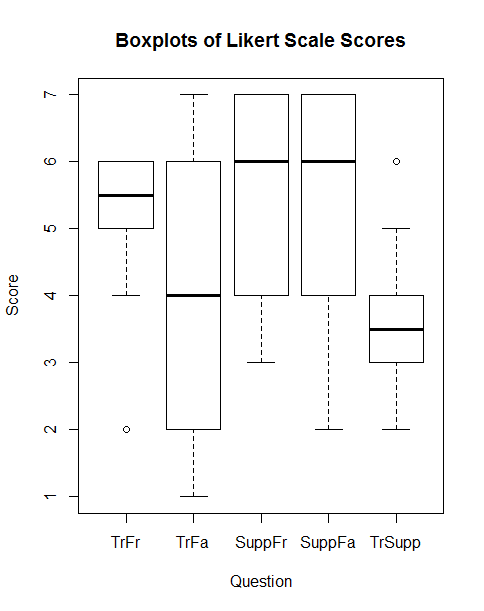
\includegraphics[width=0.6\textwidth]{likert.png}
    \caption[Likert Scale Box Plots]{
      Results of Likert scale styled questions on the opening questionnaire.
      TrFa and TrFa asked whether participants want to talk to
      Friends or Family when Troubled.
      SuppFa and SuppFa asked whether participants felt supported by
      Friends or Family.
      TrSupp asked if they reached out, in general, when troubled.
    }
    \label{fig:likert}
    \end{figure}

  Also in the opening questionnaire, we administered a Perceived Stress Scale.
  The results, shown in a histogram in Figure \ref{fig:perceived_stress},
  show that in general, the users in this study had relatively low
  self-reported stress.

    \begin{figure}
    \centering
    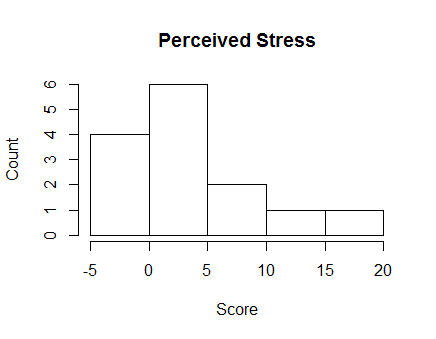
\includegraphics[width=0.6\textwidth]{perceived_stress.png}
    \caption[Perceived Stress]{
      Distribution of Perceived Stress scores amongst the 15 participants.
    }
    \label{fig:perceived_stress}
    \end{figure}

\section{Opening Interview: Script Based Results}
  The opening interview, as mentioned in Section \ref{sec:opening_int},
  followed a script, so some results were in response to scripted questions.

  \subsection{Support-Interest}
  Because the participants' situations were so different,
  the degree to which they wanted or needed social support were very different as well.
  I assessed their general degree of need and interest in reaching out,
  what I call support-interest, during the interview.
  I define support-interest as the trait of consistently having a desire
  and making efforts to
  connect on an emotional and empathetic level with loved ones.
  Based on the nature of their support network
  and how they choose to interact with the members in it,
  it is relatively straightforward to characterize the interviewee's
  current level of support-interest.
  From the interviewees descriptions, support-interest isn't an inherent trait,
  and is instead also dependent upon the current situation of the interviewee.

  Interviewees on the low support-interest end of the spectrum
  have a preference for keeping their concerns to themselves.
  Two interviewees seemed especially independent,
  expressing a desire for and general pattern of dealing with things alone,
  without much external input.
  Both reported having plenty of friends that they interacted with regularly,
  but they chose to keep them at a greater distance when it came to things
  they were particularly sensitive about.
  When asked
  about how they discuss serious subjects with those closest to them,
  they tend to express a lack of interest.
  A quote from one of them
  helps to express the sentiment:
  \begin{itemize}
  \item
  \textit{
  ``[These thoughts are] my personal complications.
  I usually don't share that much with people because
  I'm not comfortable with them knowing me too well.
  I prefer to keep a personal boundary."
  }
  - Participant 1847, on her thoughts about keeping her privacy,
  \end{itemize}

  On the high support-interest end of the spectrum, there was a lot of variability.
  High support-interest people included my married participants, who notably,
  married within the last 5 years or so,
  and expressed being very open with their spouses, sharing everything.
  They also included a participant very active in her church community,
  and other individuals close with their parents or significant others.
  These participants expressed investing a lot of time in
  sharing feelings and struggles.
  Quotes associated with them included:
  \begin{itemize}
  \item \textit{
  ``She was the first person that I felt like I could talk freely with.
  We can talk about anything and everything.
  She asks questions that really pin at trying to figure out
  where emotions are coming from, what's really bothering me at a certain time.
  Just the fact that she lets me talk freely and with understanding
  makes me more comfortable."
  }
  - Participant 8594, about her mentor figure.
  \item \textit{
  ``I talk most to my mom... I try to tell my mom everything.
  She's not pushy, but she won't let me not tell her things.
  She'll ask `And then what did the doctor say? And then?
  What's this medicine? I need to look it up!'
  [So] then I tell her everything, because she worries."
  }
  - Participant 1496, about her mother.
  \item  \textit{
  ``We're on GChat a lot.
  We chat throughout the day.
  I know how she's feeling with about a 15 minute resolution."
  }
  - Participant 3792, about his girlfriend.
  \item \textit{
  ``I have a really honest relationship with [boyfriend name].
  He'll be the first one to check in after a medical appointment,
  so is most aware...
  Rather than him trying to make sense of it,
  it makes more sense for him to just be supportive and be there.
  ... If I say anything negative, he'll jump on it.
  If I'm feeling down on myself,
  just him kinda being, `Hey, you're doing the best you can.'
  ... Sometimes I'm in the place to hear it."
  }
  - Participant 4416, about her boyfriend.
  \item \textit{
  ``I have a group of two women.. we call ourselves accountability partners.
  We meet up, like, every week.
  The idea of keeping each other accountable is
  [about] committing to listen to one another, encourage one another,
  and challenge one another to live a life of faith."
  }
  - Participant 5397, about her certain members of her church community.
  \end{itemize}

  \subsection{Choosing People and Choosing Topics}
  On discussing the support network of the interviewees,
  they tended to have a certain group of people that they turned to for
  general day-to-day support.
  These people could be family, or family-like people, as well as friends,
  but most times, participants had a strong preference towards one or the other.
  In most cases, the interviewee chose to discuss serious subjects ---
  about things that were really on their minds ---
  with only friends or only family,
  and chose to discuss only mundane, less serious topics with the other.

  For example, Participant 1010, talking about her parents,
  expressed a common sentiment.
  \textit{
  ``We only talk about mundane things...
  things not directly related to life."
  }

  \subsection{Serious Situation}
  Although the call for participant recruitment called for participants
  dealing with some serious situation in their lives,
  whether mourning or illness or other unusual difficulty of transition,
  the severity of the participants' situations varied.

  On the lighter end of the spectrum included six participants who were
  dealing with regular academic and career pressures.
  On the heavier end,
  three participants were dealing with very serious chronic illnesses,
  another was bereaved,
  and others were battling other forms of daunting transitions and trials.

  \subsection{Meeting Needs}
  Luckily, all of my participants who wanted support had people
  who could provide it.
  However, as anticipated by other research \cite{skeels10},
  when the needs grew, it became harder for some of my participants to get
  what they needed.

  Participant 9541 expressed a general sentiment about discussing tough topics:
  \textit{
  ``Feeling like you need it and actually reaching out are two different things.
  It's a lot harder to say `I'm struggling with whatever's going on.'"
  } and Participant 5397 described a high learning curve
  \textit{
  ``Two years ago.
  Actually, even a year ago, I was not very good about reaching out to people.
  It takes a lot of energy to reach out to people and explain what's going on.
  [We thought]
  `If these people are really my friends, they should be reaching out to me,'
  but actually, if they don't know, they don't know.
  Nowadays, there's a group of people we'll email or call.
  Maybe we should be asking a few people, specifically, to be on-call."
  }

  \subsection{Technology}
  Participants tended to be technically savvy.
  They were young, ranging from age 18 to 30,
  and consistent with previous research,
  they used a complex range of technologies to connect
  with friends and family near and at distance,
  for a range of complicated reasons.

  Texting and instant messaging were
  were used frequently for casual things such as keeping in touch,
  and other modes of communication, such as video, phone, or in person meetings,
  were used for more serious topics.
  The exception to this was email,
  which despite being digital and text based, 
  afforded a level of thoughtfulness that participants
  felt were especially valuable in a different way.
  Email was favored by two participants, one who wrote distant friends about
  the condition of her chronic illness,
  and the other who had depressive episodes.
  They found that email communication was more comfortable than media
  that were more immediate.

\section{Opening Interview: Other Trends}
  Many interesting results, decision patterns, and phenomena
  were not anticipated by the script.

  \subsection{Direction of Awareness}
  In many cases, there was a clear directionality to the type of awareness
  information shared.
  For example, it was common for children to report a lot to their parents,
  but the parents often shared little in return.
  This could also be true for other relationships,
  such as between siblings or friends,
  with one party in the habit of disclosing more to the other.
  A specific example was from Participant 1010:
  \textit{
  ``With some of my friends, I like to know what they're doing.
  I kinda mother them.
  I like to make sure they're doing okay."
  }

  \subsection{Extreme Information Withholding}
  Another phenomenon that became apparent with interviews is that
  many, normally trusting, close relationships,
  can exhibit information withholding.
  On the topic of awareness and updates from family,
  a rather sad event was recounted with dry laughter by Participant 2928.
  \textit{
    ``
    They don't tell me anything. No.
    They feel like I should focus on me.
    Even when my dog passed away, they didn't tell me for an entire month.
    They didn't want me to be upset.
    I just noticed the dog wasn't there, and they never straight up told me."
  }

  It's important to note that the story is one instance of a general
  trend of not sharing bad news.
  This can take the form of general reticence on the subject:
  \textit{
  ``[My struggles are] not really fun to talk about.
  Most people already have enough on their plate"
  }
  - Participant 9451
  or still discussed, but replaced by a positive spin instead:
  \textit{
  ``I try to look on the bright side.
  For example, my Facebook page used to be full of sad things.
  I decided not to do that anymore."
  } - Participant 3792
  
  This can also be taken to the extreme.
  One specific example from my participants involved
  completely not telling family members about a serious issue,
  while maintaining communications otherwise.

  \subsection{Changes in Support Structure}
  Lastly, closely related to the extreme information withholding,
  there are many situations in our lives that result in
  drastic changes in the nature of our support structure.
  As mentioned in Section \ref{sec:intro},
  death can be the most tragic cause of such a change.
  When the person who passed away had a pivotal role in the support
  structure of another, it can be even harder to cope with
  the difficult period of mourning.
  Though this was true for a participant who was bereaved,
  the drastic changes that other interviewees described usually involved
  a falling out of some sort.
  These falling outs could be between family members,
  significant others, or even friends,
  and completely overturn an existing network.

\section{Android}
  After the Opening Interview, participants were instructed to invite
  at least 2 people to join their group.
  Once there were 3 people in a group,
  they were given the InMind application,
  and they could begin the second phase of the study.

  \subsection{Attrition}
    \label{sec:Android}
    Of the 15 participants, 2 could not continue the Android portion
    of the study due to timing constraints.
    5 more did not get two people in their group,
    so after two weeks,
    we decided to call them in for a closing interview.

    The closing interview, instead of asking about the experience of using
    the application, just inquired into the reasons for not recruiting friends.
    One benign reason for failing to recruit is that users did not have friends
    who used Android phones.
    One participant asked 5 friends and discovered all were iPhone users.
    Another was that the participants simply became too busy to interact with
    friends and ask them to be in a study with them.

  \subsection{Weekly Feedback}
  During the study,
  I asked for feedback via open ended online questionnaires,
  and offered optional in-person check-ins that 3 of participants took me up on.

  Most of the weely feedback consisted of feature requests.
  Some participants wanted to be able to change the sharing status
  of a topic after it was started.
  Others wanted to be able to post pictures onto a topic.
  A full compiled list of feature requests has been compiled in Appendix B.

  In general, the suggestions were reflective of the users' experience with other
  applications for communication, such as Google Hangouts \cite{gchat},
  Line \cite{line}, or QQ \cite{QQ},
  in that users expected to be able to send pictures, emoticons, video,
  and receive notifications for messages.

  On the other hand, one participant contrasted the slow messaging design with
  the other forms of communication she was more used to,
  and said she liked knowing that the other
  people in the group weren't being immediately contacted when she wrote messages.

  \subsection{Affective Benefits and Costs Questionnaire}
  The Affective Benefits and Costs Questionnaire (ABC-Q) as described in
  the Study section, is intended to measure various factors
  related to the usage of a communications technology.
  
  Figure \ref{fig:abcq_results} shows the scores,
  over 3 weeks, that the participants reported.
  Once I drop the outlier data point, Participant 1847,
  the the average ABC-Q scores reported by participants hold at a steady positive 13
  for all three weeks.

    \begin{figure}
    \centering
    \includegraphics[width=0.6\textwidth]{abcq_scores.jpeg}
    \caption[Affective Benefits and Costs Questionnaire Results]{
      Over 3 weeks, the ABC-Q scores reported by participants tended to vary
      a little.
      The outlier may be due to bad reporting.
    }
    \label{fig:abcq_results}
    \end{figure}

  Note: The outlier participant, visible in Figure \ref{fig:abcq_results}
  as changing extremely from very positive,
  to very negative, and back to very positive may have had reporting errors.
  Her questionnaire's subscores reported that in the second week,
  she felt that the application invaded her privacy.
  I brought up the topic of privacy during our closing interview, and she reponded,
  \textit{
  ``I don't think it invaded my life. It was a very optional thing,
  if I wanted to use it, I used it. Maybe I submitted a bad feedback.
  I don't think it's an invasion of privacy."
  }

  \subsection{System Usability Scale}
  The system
  This distribution of System Usability Scores (SUS) is shown in figure
  \ref{fig:sus_results}.
  The SUS is scored from 0 to 100, but the average score for the SUS is 68,
  so we compare our results to that.
  A students t-test of the average score of the data, minus an outlier,
  is significantly  different from the expected average of 68 (p=0.0136),
  suggesting that InMind is doing reasonably well in usability.

    \begin{figure}
    \centering
    \includegraphics[width=0.3\textwidth]{sus_boxplot.jpeg}
    \caption[System Usability Scale Results]{
      System Usability Scores included an outlier,
      but was otherwise centered around 72,
      and is significantly different (p=0.0136) from the expected average of 68.
    }
    \label{fig:sus_results}
    \end{figure}

\section{Data from Application}
  Since the data set only includes 8 groups,
  it is not particularly meaningful to derive any statistical conclusions
  from them.
  However, a data set of 36 users, 70 topics, and 1043 messages
  is still useful for observing some likely trends.
  The questions that I will discuss in this section address
  permissions given to topics, the life cycle of a topic,
  user interactions over 3 weeks of usage,
  and variability between the 8 groups.

  \subsection{Permissions}
  An important question posed at the beginning of this study
  considered the privacy level of topics.
  The hypothesis was that for many serious topics,
  the privacy of the information was very important to the owner of the topic,
  so the owner would want to control who had access to it.
  In this study, of the 70 topics observed, 13 were shared with no-one,
  and were used by the owners to organize their own thoughts.
  27 topics were shared with "Everyone" within the group,
  and the remaining 30 were shared with some subset of people.
  It is safe to assume from this usage data that
  there is a desire to organize tihngs for oneself,
  and the topics that are shared are roughly evenly distributed
  between those that the owner is fairly comfortable sharing with the public,
  and those that are shared with specfic people.

  \subsection{Topic Life Cycle}
  Topics are created generally in the mornings and evenings,
  presumably before the day starts and after the day ends,
  and not when things are happening.
  The distribution of hours of creation is shown in
  Figure \ref{fig:topic_hours},
  which shows a bimodal distribution centered on waking and sleeping hours.

  \begin{figure}
  \centering
  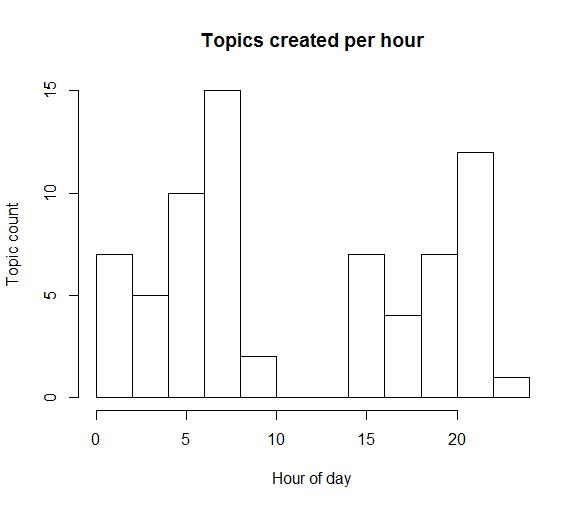
\includegraphics[width=0.6\textwidth]{topics_per_hour.jpg}
  \caption[Topics Created by Hour of Day]{
    Topics were created at varying hours of the day.
    The 70 topics shown in this bar chart appear to show
    topics being created in the morning and evenings,
    and occasionally in late evening/early morning,
    but fewer in the middle of the day, between 10:00 A.M. and 3:00 P.M.
  }
  \label{fig:topic_hours}
  \end{figure}

  After the opening interviews, we considered the types of stressors the
  interviewees faced, and postulated two likely types of topics.
  short lived and long lived ones.
  Short lived topics we imagined would last a few days to a week,
  and would include things like class projects,
  work deadlines, short conflicts with friends, and other temporary frustrations.
  Long lived topics we imagined would last much longer,
  and would include the more chronic, serious topics,
  and since these stressors can last from several months to indefinitely,
  they should remain active for the duration of the 3 week study.
  This ended up remarkably accurate,
  but we had not anticipated that many topics would be created,
  and never become active.
  These ``zero-day" topics were created,
  but were neither updated nor discussed after the day they were created.
  Explanations from the interviews general expressed a lack of interest
  in the topic after the initial posting.

  In Figure \ref{fig:topic_age}, charts show two different measures of 
  topic duration, filtered and not filtered to remove the zero-day topics.

  \begin{figure}
  \centering
    \begin{subfigure}[b]{0.4\textwidth}
      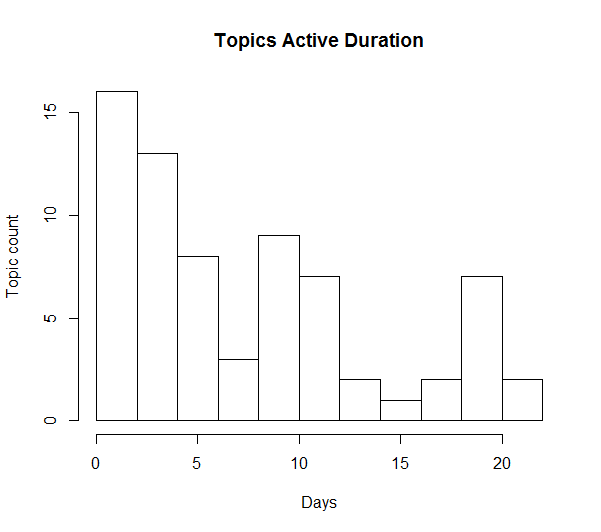
\includegraphics[width=\textwidth]{topic_days_active.png}
      \caption{Days topics were discussed after creation.}
    \end{subfigure}
    \begin{subfigure}[b]{0.4\textwidth}
      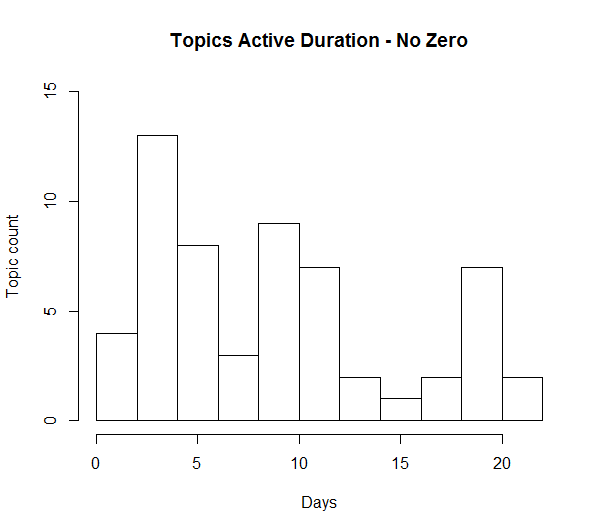
\includegraphics[width=\textwidth]{topic_days_active_nz.png}
      \caption{Days topics were discussed after creation,
        minus topics not discussed after the first day.}
    \end{subfigure} \\
    \begin{subfigure}[b]{0.4\textwidth}
      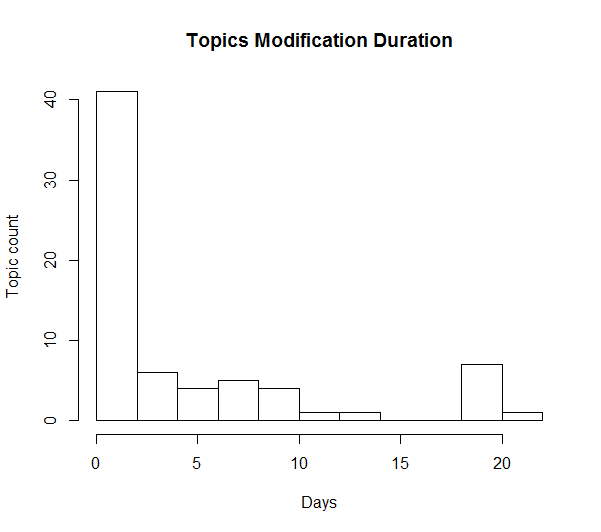
\includegraphics[width=\textwidth]{topic_days_mod.png}
      \caption{Days topics had status changed, after creation.}
    \end{subfigure}
    \begin{subfigure}[b]{0.4\textwidth}
      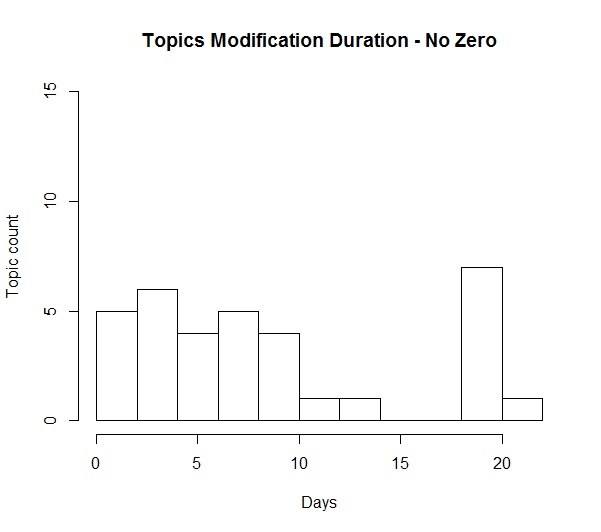
\includegraphics[width=\textwidth]{topic_days_mod_nz.png}
      \caption{Days topics had status changed, after creation, minus zeros.}
    \end{subfigure}
  \caption[Duration of Topics] {
    Topics were active for varying periods.
    Note that there are so many topics that did not have their status changed
    after the first day that the vertical scale is greater on subgraph c.}
  \label{fig:topic_age}
  \end{figure}

  \subsection{General Usage During Study}
    The number of topics created and number of messages sent changed over
    the course of the 3 weeks.
    Counts of how many of each occurred each week are summarized in
    Table \ref{table:weekly}
    On average, each group created about 5 topics the first week,
    2 topics the second week, and 1 topic the third week,
    and similarly, sent 70, 45, and 15 messages.
    This pattern was explained by the users in the closing interviews.
    The first week or so saw heavy usage because users had to inform
    people within the group about both long and short term topics,
    as they were all newly introduced into the application.
    Then, after some time, usage stabilzed to a few updates to long term topics,
    and occasionally a new topic.
    We can reasonably postulate that the 3rd week's usage is much more likely
    to be that demonstrated by users in the long term,
    but the study duration was not long enough to get to a stable equilibrium.

    \begin{table}[h]
    \centering
    \caption{Weekly Activity}
    \label{table:weekly}
    \begin{tabular}{ l l l}
    Week & Topics Created & Messages Sent \\
    \hline
    1 & 43 & 558      \\[5pt]
    2 & 17 & 361      \\[5pt]
    3 & 10 & 124      \\[5pt]
    \hline
    Total & 70 & 1043       \\[5pt]
    \end{tabular}
    \end{table}

  \subsection{Variability Between Groups}
    The variability between groups is best explained by the
    qualitative contents of the closing interview,
    but the data gives us a preview.
    Looking at the number of messages sent within a group,
    we see that a likely typical number of messages sent within a group
    is between 30 and 100,
    but there is an outlier of more than 600 messages in one group.

    \begin{figure}
      \centering
      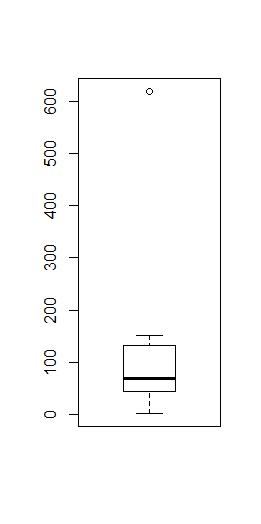
\includegraphics[width=0.3\textwidth]{messages_per_group.jpeg}
      \caption[Messages Sent by Groups]{
        The number of messages sent by each group varied between
        2 and an outlier at more than 600 messages.
      }
      \label{fig:topic_hours}
      \end{figure}

\section{Closing Interview}
  The closing interview also followed a script,
  and similarly to the opening interview, some themes quickly bubbled up from
  beyond the explicit content of the questions in the script.

  \subsection{Positive Experiences: Unique Usage Methods}
    The positive experiences were mostly reported by the people
    whose groups sent a total of more than 100 messages.
    Each of these groups found their own unique way of making the topic-based
    communication work for them.

    \subsubsection{Day-Logging}
    The group with the heaviest usage, over 600 messages in the course of 3 weeks,
    was the group surrounding Participant 5397.
    Suffering from a chronic illness,
    Participant 5397 was interested in logging her day to day activities,
    food consumption, and wellness.
    \textit{
    `` I have one topic about my diet, and foodstuff, and another that was on
    how I'm doing or feeling, and those would be the ones I'd update
    even if no-one had said anything. Typically my friend was very good about making some sort of comment,
    so I'd be reponding to her, but I'd also just update it."
    }

    Several features of Participant 5397's habits suggest why her and her group's
    usage was so high.
    In the second week, she said, 
    \textit{``I've become more accustomed to working with InMind and had somewhat
    of a ``schedule" (a very loose one) to check it before bed,
    which coincided somewhat nicely with my nightly reflection time.
    [T]he active group member has been asking me questions that might not come up
    in our typical interactions...
    This kind of daily back and forth has developed our friendship
    and made me think more."}
    This suggests a regular schedule and habit of reflection,
    and that InMind integrated smoothly with her existing habits,
    and that she got value out of having someone being on the other end,
    responding and reflecting with her.

    Further, during the closing interview, she described InMind as a convenient
    way to send logs to other people every day,
    as opposed to other forms of communication, such as email, in which she sends
    one email a week at best.
    When asked about comparing InMind updates to her weekly emails.
    \textit{
    ``The two different formats of email vs status messages are good for different
    things.
    One of them is weekly. One of them is daily.
    The emails weren't as minute in terms of details.
    In the app, it doesn't encourage long messages,
    so I updated more as if it were a Twitter feed."
    }

    \subsubsection{Self-Reflection}
    The second most active group was associated with Participant 8597.
    She reported early on that her friends weren't really involved in her group,
    and didn't seem to find a use for InMind, but she did.
    Participant 8594 used it for regular self reflection,
    and found personal value in using it.
    \textit{``It has helped me keep an overview of everything on my mind,
    and it let's me try to be more honest with how I assess my feelings
    on each thing."}
    
    \subsubsection{Activity Sharing}
    Finally, the last group that had over 100 messages was that of
    Participant 1674.
    His group's advantage was that the participants in the group were all
    more active on InMind.
    Thus, there was generally more interaction,
    and the activities were not as individually driven.
    The members of his group were in his research group,
    and they were sharing some common stressors that they could come together on.
    Further, they also were traveling together,
    and there were logistical/experience-based communications that were
    valuable for the members in the group.

  \subsection{Negative Experiences: Limitations of Study Deployment}
    \subsubsection{Sparse Interaction}
      When asked about negative experiences, 5 of the 8 participants
      described, in various ways, the disappointment associated with
      a lack of interaction from the other members within the group.
      The disappointment came specifically from instances when members of the group
      did not respond to messages sent through InMind.

      This was due to two primary reasons.
      The first reason, which applied to 1 of the 5 people,
      reflected that he expected much faster message turnover rate,
      and that for him,
      more timely responses are more useful for him, and getting a message
      several hours/a day after the incident is not helpful.
      The second reason, is related to the people in the group.
    \subsubsection{Group Membership}
      At the end of the study, when I compared the descriptions of the members
      of their actual research group with the people they reported as close
      to them during the opening interview,
      I realized that in all but 1 of the 8 groups,
      the members of the group were not people the participant would normally
      go to for support.

      In some cases, this was discovered when I asked about the membership of
      the participants' groups.
      Besides them being not being the people
      that the participants felt close to, they also tended to respond less.
      \textit{``I wish that the people I invited in could have done more."}
      - Participant 8597.

      The group for which the members were actually likely to be sources of support
      for the participant was that of Participant 1674.
      His group of coworkers were very close, and their interactions were
      thus the most balanced of the 8 groups.

      Besides them, every single other group was composed of
      the participant and 2 or 3 people somewhat arbitrarily drawn from
      their pool of acquaintances, based on the requirement that
      they own an Android phone.
      This is primarily a result of the study limitation imposed by requiring
      an Android device for admittance into the group,
      and it severely limited the depth of interaction possible over InMind.
      In the end, the value of the application depends on the value
      of the connections it supports.
      In one group (that of Participant 5397), it rekindled a relationship
      between the participant and an old friend,
      but in most of the groups, without existing strong ties,
      there really just wasn't much that anyone wanted to share.

  \subsection{Support Needs and Topics}
    The participants did not report any significant changes in the stressors
    in their lives,
    though the intesity of the stressors varied over the course of the 3 week study.
  
  \subsection{Meeting Needs: Dependence Upon Group Members}
    Related to the fact that relationships between members of the groups
    were not particularly strong,
    most of the time InMind was not used to explicitly reach out for support.
    I believe that it is due to the lack of confidence in getting a response
    from the group,
    but most consistent interactions within a group were for personal purposes,
    so instead of encouraging the actions of reaching out for help
    it seems to have encouraged self-organization and independence instead.

  \subsection{Interaction With Other Technologies}
    This topic resulted in varied results.
    Some groups (4 out of 8) brought topics from within the application to outside
    of it, via text messages, emails, or phone calls,
    and InMind functioned as an initiator for conversations.
    In many ways, this was the primary function of InMind,
    to give serious topics a place in the minds of the relevant close ties,
    and allow them to bring it up over richer communication pathways.

    For 3 out of the 8 groups, not so coincidentally the lower usage rate groups,
    topics that existed within InMind stayed within InMind,
    and never made it into the participants other interactions with their group
    members.

\chapter{Conclusion}
\section{TBD}

\appendix
\chapter{Additional Materials}

\clearpage
\newpage

\chapter{Data}
\section{Questionnaire}

\subsection{ABC-Q Responses}
  \begin{table}
  \end{table}

\subsection{Weekly Questionnaires}
  In the weekly questionnaires, when we asked for general feedback,
  we got a lot of feature requests instead.

  \begin{enumerate}
  
  \end{enumerate}

\subsection{ABC-Q Responses}
  \begin{table}
  \end{table}

\section{Database}
\label{sec:appb_data}
\vspace*{-3in}
    \renewcommand{\arraystretch}{1.2}
    \begin{table}
    \centering
    \begin{tabular}{  l  l  l }
    \hline
    Collection & Fields & Type \\
    \hline
    Groups
    & group\_id & String \\
    & IV & String \\
    & members & array of Strings \\
    \hline
    Users
    & alias & String \\
    & is\_lead & Boolean \\
    & passphrase & String \\
    & user\_id & String \\
    \hline
    Topics
    & archived & Boolean \\
    & color & Integer \\
    & group\_id & String \\
    & modified\_at & Date \\
    & owner & String \\
    & passphrase & String \\
    & salt & String \\
    & shared\_with & array of Strings \\
    & smiles & Integer \\
    & state & Integer \\
    & title & String \\
    & type & String \\
    \hline
    Messages
    & owner & String \\
    & topic & String \\
    & text & String \\
    \end{tabular}
    \caption[Datatypes in DB]{
    All datatypes in the database have a unique id and a created\_at date,
    in addition to the fields listed.}
    \label{fig:api_table}
    \end{table}

\section{App Analytics}


\clearpage
\newpage

\begin{thebibliography}{25}

\bibitem{mikal13}
  Jude P. Mikal, Ronald E. Rice, Audrey Abeyta, Jenica DeVilbiss.
  2013.
  \emph{Transition, stress and computer-mediated social support}
  Computers in Human Behavior 29.5 (2013): A40-A53.

\bibitem{rains09}
  Rains, Stephen A., and Valerie Young.
  \emph{A Meta-Analysis of Research on Formal Computer-Mediated Support Groups: Examining Group Characteristics and Health Outcomes.}
  Human Communication Research 35.3 (2009): 309-336

\bibitem{shor13}
  Shor, Eran, David J. Roelfs, and Tamar Yogev.
  \emph{The strength of family ties: A meta-analysis and meta-regression of self-reported social support and mortality.}
  Social Networks 35.4 (2013): 626-638.

\bibitem{lehman86}
  Lehman, Darrin R., John H. Ellard, and Camille B. Wortman.
  \emph{Social support for the bereaved: Recipients' and providers' perspectives on what is helpful.}
  Journal of Consulting and Clinical Psychology 54.4 (1986): 438.

\bibitem{vachon88}
  Vachon, Mary LS, and Stanley K. Stylianos.
  \emph{The role of social support in bereavement.}
  Journal of Social Issues 44.3 (1988): 175-190.

\bibitem{shaw02}
  Shaw, Lindsay H., and Larry M. Gant. 
  \emph{In defense of the Internet: The relationship between Internet communication and depression, loneliness, self-esteem, and perceived social support.}
  CyberPsychology \& Behavior 5.2 (2002): 157-171.

\bibitem{hjo14}
  Oh, Hyun Jung, Elif Ozkaya, and Robert LaRose.
  \emph{How does online social networking enhance life satisfaction? The relationships among online supportive interaction, affect, perceived social support, sense of community, and life satisfaction.}
  Computers in Human Behavior 30 (2014): 69-78.

\bibitem{mm11a}
  Massimi, M. and Baecker, R.M.
  \emph{Dealing with death in design: Developing systems for the bereaved.}
  Proc. ACM SIGCHI 2011, 1001-1010

\bibitem{mm10}
  Michael Massimi and Ronald M. Baecker.
  2010.
  \emph{A death in the family: opportunities for designing technologies for the
  bereaved.}
  In Proceedings of the SIGCHI Conference on Human Factors in Computing
  Systems (CHI '10).
  ACM, New York, NY, USA, 1821-1830. 

\bibitem{mm13}
  Michael Massimi.
  2013.
  \emph{Exploring remembrance and social support behavior in an online
  bereavement support group.}
  In Proceedings of the 2013 conference on Computer supported cooperative
  work (CSCW '13). ACM, New York, NY, USA, 1169-1180. 

\bibitem{brubaker11}
  Jed R. Brubaker and Gillian R. Hayes.
  2011.
  \emph{"We will never forget you [online]"}
  In Proceedings of the ACM 2011 conference on Computer supported cooperative
  work
  (CSCW '11). ACM, New York, NY, USA, 123-132. 

\bibitem{neustaedter12}
  Carman Neustaedter, Steve Harrison, and Abigail Sellen.
  2012.
  \emph{Connecting Families: The Impact of New Communication Technologies on
  Domestic Life.}
  Springer Publishing Company, Incorporated.

\bibitem{neustaedter06}
  Carman Neustaedter, Kathryn Elliot, and Saul Greenberg.
  2006.
  \emph{Interpersonal awareness in the domestic realm.}
  In Proceedings of the 18th Australia conference on Computer-Human Interaction:
  Design: Activities, Artefacts and Environments (OZCHI '06),
  Jesper Kjeldskov and Jeni Paay (Eds.). ACM, New York, NY, USA, 15-22.

\bibitem{markopoulos04}
  Panos Markopoulos, Natalia Romero, Joy van Baren, Wijnand IJsselsteijn,
  Boris de Ruyter, and Babak Farshchian.
  2004.
  \emph{Keeping in touch with the family: home and away with the ASTRA awareness
  system.}
  In CHI '04 Extended Abstracts on Human Factors in Computing Systems.
  ACM, New York, NY, USA, 1351-1354.

\bibitem{pollack11}
  John P. Pollak, Phil Adams, and Geri Gay.
  2011.
  \emph{PAM: a photographic affect meter for frequent, in situ measurement of
  affect.}
  In Proceedings of the SIGCHI Conference on Human Factors in Computing Systems
  (CHI '11). ACM, New York, NY, USA, 725-734. 

\bibitem{mm11b}
  Michael Massimi.
  2011.
  \emph{Technology and the human lifespan: learning from the bereaved.}
  interactions 18, 3 (May 2011), 26-29.

\bibitem{hassenzhal12}
  Marc Hassenzhal, Stephanie Heidecker, Kai Eckoldt, and Satah Deifenbach.
  2012.
  \emph{All You Need is Love: Current Strategies of Mediating Intimate
  Relationships through Technology}
  ACM Transactions on Computer-Human Interaction, Vol. 19, No. 4, Article 30

\bibitem{vetere05}
  Frank Vetere, Martin R. Gibbs, Jesper Kjedskov.
  2005.
  \emph{Mediating Intimacy: Designing Technologies to Support
  Strong-Tie Relationships}
  CHI 2005, April 2�7, 2005, Portland, Oregon, USA.

\bibitem{lottridge09}
  Danielle Lottridge, Nicolas MAsson, Wendy Mackay
  2009.
  \emph{Sharing Empty Moments: Design for Remote Couples}
  CHI 2009, April 4�9, 2009, Boston, MA, USA.

\bibitem{octavia07}
  Johanna Renny Octavia, Elise van den Hoven, Hans De Mondt.
  2007
  \emph{Overcoming the Distance Between Friends}
  HCI 2007, 3-7 September 2007, Lancaster University, UK.

\bibitem{brush08}
  A.H. Bernhein Brush, Kori M Inkpen, Kimberly Tee.
  2008.
  \emph{SPARCS: Exploring Sharing Suggestions
  to Enhance Family Connectedness}
  CSCW�08, November 8�12, 2008, San Diego, California, USA.

\bibitem{morris04}
  Morris, Margaret, Jay Lundell, and Eric Dishman.
  \emph{Catalyzing social interaction with ubiquitous computing: a needs assessment of elders coping with cognitive decline.}
  CHI'04 extended abstracts on Human factors in computing systems. ACM, 2004.

\bibitem{skeels10}
  Meredith M. Skeels, Kenton T. Unruh, Christopher Powell, Wanda Pratt.
  2010.
  \emph{Catalyzing Social Support for Breast Cancer Patients}
  CHI 2010, April 10�15, 2010, Atlanta, Georgia, USA

\bibitem{luxton11}
  Luxton, David D., et al.
  \emph{mHealth for mental health: Integrating smartphone technology in behavioral healthcare.}
  Professional Psychology: Research and Practice 42.6 (2011): 505.

\bibitem{patil05}
  Patil, Sameer, and Jennifer Lai. 
  \emph{Who gets to know what when: configuring privacy permissions in an awareness application.}
  Proceedings of the SIGCHI conference on Human factors in computing systems. ACM, 2005.

\bibitem{gchat}
Google Talk (Hangouts)
\url{http://www.google.com/hangouts/}

\bibitem{line}
LINE
\url{http://line.me/en/}

\bibitem{QQ}
QQ International
\url{http://www.imqq.com/}

\bibitem{parkes13}
Parkes, Colin Murray, and Holly G. Prigerson. Bereavement: Studies of grief in adult life. Routledge, 2013.

\end{thebibliography}

\end{document}

